\documentclass[12pt]{article}
\usepackage[a4paper, margin=2cm]{geometry}
\usepackage[english]{babel} % To obtain English text with the blindtext package
\usepackage{blindtext}
\usepackage{graphicx} % Required for inserting images
\usepackage{array, multirow} % For extra column formatting
\usepackage{amsmath, amssymb, cancel} %for equation environment
\usepackage{float}
\usepackage{parskip} % For gaps between para
\usepackage{setspace}
\usepackage{pdfpages}
\usepackage{abstract}
\usepackage[export]{adjustbox}
\usepackage{emptypage}
\usepackage{tocloft}
\usepackage[nottoc]{tocbibind}
\usepackage{hyperref, url}
\usepackage[table]{xcolor}
\usepackage{minted}
    \usemintedstyle{monokai}
\usepackage{caption,subcaption}
    \captionsetup{font=footnotesize,labelfont=bf}
    \subcaptionsetup{font=footnotesize}
\usepackage{tcolorbox}
    \newtcolorbox{mintedbox}{
        colback=backcolour,
        boxrule=0pt,
        sharp corners,
        width=\linewidth,
        left=0pt, right=0pt,
        top=3pt, bottom=3pt
    }

\cftsetindents{section}{0em}{2em}
\cftsetindents{subsection}{0em}{2em}

\renewcommand\cfttoctitlefont{\hfill\Large\bfseries}
\renewcommand\cftaftertoctitle{\hfill\mbox{}}

\graphicspath{ {./images/} }

\definecolor{blurple}{HTML}{5865F2}
\definecolor{backcolour}{HTML}{272823}

\hypersetup{
    colorlinks=true,
    linkcolor=black,
    urlcolor=black,
    citecolor=blurple,
}

\urlstyle{same}

\renewcommand{\arraystretch}{1.3}

\setcounter{secnumdepth}{5}
\setcounter{tocdepth}{5}
\newcommand\simpleparagraph[1]{%
  \stepcounter{paragraph}\paragraph*{\theparagraph\quad{}#1}}

%%%%%%%%%%%%%%%%%%%%%%%%%%%%%%%%%%%


\title{PHYC20040 Exp.9 Holography}
\author{Joana Adao}
\date{\today}

\begin{document}

\begin{titlepage}
    \begin{center}

        \begin{figure}[ht]
            \includegraphics[width=\textwidth]{UCDLogo.png}
        \end{figure}
        
        \begin{figure}
            \centerline{\includegraphics[width=\paperwidth]{UCDBanner.png}}
        \end{figure}

        \vspace{4cm}

        {\LARGE \bfseries PHYC20090 Electronics and Devices}\\
        \vspace{0.75cm}
        {\Large Experiment No.9 Holography}
        
        \vspace{1cm}
    
    {\Large \textbf{24 February 2025}}

    \vspace{2cm}
    
    {\large \textbf{by Joana C.C. Adao (Student No. 23311051)}}\\
    \medskip
    {\large With Ananya L.}

    \end{center}
    
   \clearpage

\end{titlepage}

\setcounter{page}{1}
\tableofcontents
\pagenumbering{roman}

\newpage

\begin{abstract}
\addcontentsline{toc}{section}{Abstract}
\pagenumbering{arabic}

Holography is a technique that is able to record and reconstruct wavefronts of light in order to create a three-dimensional replica of an object. The aim of this experiment was to explore
the principles and concepts of holography by recording and developing a reflection hologram with red laser light. This process was done with carefully assembled apparatus to be able to properly develop the 
interference patterns that are fundamental to the creation of 3D hologram. The final result was a high quality, clear, and sharp hologram of a key that accurately recreated the object's shape, depth, and texture
with notable variations in intensity that capture the effect of light on the surface at the moment of recording. This experiment successfully desmonstrated Bragg diffraction seen in reflection holograms and
the necessity of using a laser light for holography due to its monochromaticity, coherence, intensity, and directionality properties. Holography was then explored for use in the medical field, data storage, and in
augmented/virtual reality devices.

 
\end{abstract}

%%%%%%%%%%%%%%%%%%%%%%%%%%%%%%%%%%%

\vspace{4.5cm}

\section{Theory} \label{sec:1}

\subsection{Recording and Reconstruction of Holograms}

Holography is a technique that can record and reconstruct an image based on the "total information" content of the light (wavefronts of light) scattered by the object. These are the basic parameters that describe the light,
wavelength, amplitude, phase, polarisation, and velocity. For holography, only the phase and amplitude of the light are recorded. This process can be understood via Fourier transforms (see §\ref{sec:1.3})
\cite{UCDholo,basicholo1,princetonholo,collier2013optical}.
Visually, the hologram can be described as being as a diffraction screen that diffracts light in such a manner that accurately reconstructs the original object when suitably illuminated
\cite{basicholo1}.
The phase and amplitude information is preserved by a "reference beam" and its interference with the light being reflected off the object's surface
\cite{UCDholo,princetonholo}.

\textbf{Recording} a hologram requires the presence of the "object beam", which illuminates the object and reflects onto the recording material (typically an emulsion photographic plate for optical holography), and the
"reference beam", the light from an apparent source that shines directly onto the recording material
\cite{UCDholo,basicholo1} (see Figure \ref{fig:1}).
These beams interfere to create an interference pattern that is recorded onto the recording material (see Figure \ref{fig:2}). Precise positioning of the laser source, beam splitter, mirrors, and emulsion photographic plate is necessary as it determines the
fringe spacing of the interference pattern. Therefore misalignmnets affect the clarity and resolution of the final hologram
\cite{UCDholo,collier2013optical}.

\begin{minipage}{.49\textwidth}
    \captionsetup{hypcap=false}
    \centering
    \includegraphics[width=\linewidth]{hologram construction.png}
    \captionof{figure}{\centering Diagram of setup to record a hologram. \protect\cite{holoimg1}.}
    \label{fig:1}
\end{minipage}
\hfill
\begin{minipage}{.49\textwidth}
    \captionsetup{hypcap=false}
    \centering
    \includegraphics[width=\linewidth]{holo interference.jpg}
    \captionof{figure}{\centering Interference patterns from shifted grating superposition. \protect\cite{kafri1990physics}.}
    \label{fig:2}
\end{minipage}

\textbf{Reconstructing} a hologram is through diffraction, and it is found that the spacing of the interference fringe are of the correct size (typically between 0.4 to 0.7 microns) to give the desired diffratcion effects 
\cite{UCDholo}.
The resulting wave structure is then identical to the original, a reconstruction of the original object in 3D detail.
A "reconstructing beam", typically the original source reference beam or light of similar coherency, illuminating the photographic plate in the direction of the original source is what allows one to be able to see the hologram
\cite{UCDholo}.
The reconstructed can be seen moving through parallax effects when the angle of viewing is shifted. The existence of this parallax is what indicated whether the object has three-dimensions \cite{UCDholo}.

\vspace{1cm}

\subsection{Amplitude and Phase} \label{sec:1.2}

Tradiotional photography methods differ from holography in the sense that with holography the phase information is also retrieved, unlike photography where only spatial distribution of light intensity (amplitude) is considered which
is averaged over all phases of light \cite{collier2013optical}.

The \textbf{amplitude} of a wave is defined as the max displacement of the wave \cite{britlight}.
For a hologram the amplitude variations will affect primarily the contrast of the recorded interference pattern, influencing the final hologram quality \cite{UCDholo,latychevskaia2009simultaneous}.
Most hologram reconstruction methods assume pure amplitude, but most real-life objects affect amplitude scattering and are therefore wavelength-dependent, 
meaning amplitude is essential for accurate holographic image reconstructions \cite{latychevskaia2009simultaneous}.

The \textbf{phase} of a wave determines where the electric field is in an oscillation cycle \cite{Paschotta_2018_optical_phase}.
The optical wave can be described with a phasor (complex amplitude), which relates the optical phase to the complex phase. 
A plane wave propagating in the z-direction can be described with $Ae^{i(\omega t - kz)}$ (see §\ref{sec:1.3}).
Interference strongly depends on optical phases \cite{Paschotta_2018_optical_phase}.
It is the phase encodement that makes a hologram appear to have a three-dimensional structure due to the phase differences in the interference pattern \cite{Paschotta_2018_optical_phase}.

\begin{figure}[H]
    \centering
    \includegraphics[width=.5\textwidth]{amplitude v phase contrast.jpg}
    \caption{\centering Comparison of amplitude (a-b) and phase (c-d) contrast in holography. Modeled phase images (e) and cross-sections (f) of experimental (c) phase images \protect\cite{ampvphaseimg}.}
    \label{fig:6}
\end{figure}

The difference between the amplitude and phae contrasts in holography are depicted in Figure \ref{fig:6}, comparing the experimental (a-d) and modeled (e) reconstructions.
Amplitude contrast images (3a-b) show variations in intensity (amplitude) which affects the trasmittance ratio, while phase contrast images (3c-d) show variations in phase (phase shifts), affecting the structural reconstruction accuracy \cite{latychevskaia2009simultaneous,ampvphaseimg}.
The modeled image (3e) illustrates how amplitude and phase contribute to the final reconstruction of the holographic image, with the phase graph (3f) showcasing the spatiotemporal evolution of the phase shift \cite{ampvphaseimg}.

\subsection{Fourier Transforms} \label{sec:1.3}

Consider the reflected waves as seen in Figure \ref{fig:3}. The detailed nature of this "object beam" is dependent on the object's shape and surface
characteristics. Taking a general approach, describe the object beam as a superposition (combination) of plane waves,

\vspace{-2ex}
\begin{gather*}
    \psi_0 (r,t) = A_0 \iint F_0 (k_x,k_y) e^{i(\omega t- k_x x- k_y y - k_z z)} dk_x dk_y 
\end{gather*}

where $(k_x^2 + k_y^2 + k_z^2)^{1/2} = k = \lambda / 2$. Suppose we have permitted this wave $\psi_0$ to interfere with a reference beam given by

\vspace{-2ex}
\begin{gather*}
    \psi_1 (r,t) = A_1 e^{i(\omega t - kz)}
\end{gather*}

and have recorded the resulting intensity pattern on a photographic plate positioned in the plane $z = 0$. The intensity recorded on the plate is then

\vspace{-2ex}
\begin{gather*}
    I(x,y) = \lvert A_1 + A_0 \iint F_0 (k_x,k_y) e^{-i(k_x x + k_y y)} dk_x dk_y \rvert^2
\end{gather*}

Expanding the right-hand side of this equation, we will have terms proportional to $\lvert \psi_0 \rvert^2$, $\lvert \psi_1 \rvert^2$, and $\lvert \psi_0 \psi_1^* \rvert$.

Assuming that the reference beam is much more intense than the object beam (ie. $\lvert \psi_1 \rvert \gg \lvert \psi_0 \rvert$), then the term in $\lvert \psi_0 \rvert^2$ can be ignored,
and the intensity can be approximated as

\vspace{-2ex}
\begin{gather*}
    I (x,y) \approx \lvert A_1 \rvert^2 + A_0 A_1^* \iint F_0 (k_x,k_y) e^{-i(k_xx + k_yy)} dk_x dk_y + A_1 A_0^* \iint F_0 (k_x,k_y) e^{+i(k_xx + k_yy)} dk_x dk_y
\end{gather*}

The transmission function for a developed plate can be expressed as $T(x,y) = 1 - \gamma I(x,y)$ where $\gamma$ is a function of the exposure and
developing processes. Therefore, the hologram's transmission function is

\vspace{-2ex}
\begin{gather*}
    T(x,y) = C_0 - \gamma A_0A_1^* \iint F_0 (k_x,k_y) e^{-i(k_xx+k_yy)} dk_x dk_y - \gamma A_1 A_0^* \iint F_0 (k_x,k_y) e^{+i(k_xx +k_yy)} dk_x dk_y
\end{gather*}

where $C_0$ is a constant. Essentially, the hologram contains both scaled versions of the two-dimensional Fourier tranform of the object beam and its inverse, superimposed on each other.
When this hologram is illuminated with a plane wave life the originall reference beam, another Fourier transformation occurs, which leads to

\vspace{-2ex}
\begin{gather*}
    \psi (r,t) = \iint F(k'_x,k'_y) e^{i(\omega t - k'_xx - k'_yy - k'_zz)} dk'_x dk'_y
\end{gather*}

where, according to Fourier optics,

\vspace{-2ex}
\begin{gather*}
    F(k'_x,k'_y) = \left( \frac{1}{2 \pi} \right)^2 \iint T(x,y) e^{i(k'_xx + k'_yy)} dxdy
\end{gather*}

The three terms that make up $T(x,y)$ obligingly integrate as delta functions (unlike the ignored $\lvert \psi_0 \rvert^2$ term, which would not behave as such), and we find

\vspace{-2ex}
\begin{gather*}
    F(k'_x,k'_y) = - \gamma A_1^* A_0 F_0 (k'_x,k'_y) - \gamma A_1 A_0^* F_0^* (-k'_x, -k'_y) + C_0 \delta (k'_x)\delta(k'_y)
\end{gather*}

As a result, when the hologram is illuminated correctly (as in Figure), the emerging wave consists of three parts: (left) a term that is proportional to the original object beam, effectively
reconstructing the object in all details of amplitude and phase; (centre) a so-called "twin reconstruction" or "twin image", which can be shown to be the original object beam, reflected across the
photographic plate and travelling backwards in time; and (right) an undeflected segment of the reference beam travelling along the z-axis.

\begin{figure}[H]
    \centering
    \includegraphics[width=.7\textwidth]{holography1.png}
    \caption{\centering Two-dimensional projection of the interference patterns produced. A photographic plate at P1 would result in a transmission hologram.
    A photographic plate at P2 wiuld result in a reflection hologram. \protect\cite{princetonholo}}
    \label{fig:3}
\end{figure}

\subsection{Properties of Laser Light in Holography}

Holography relies on the properties of laser light in order to reconstruct and record the necessary three-dimensional images. Lasers are \textbf{highly monochromatic, coherent, intense, and coherent} which allows for stable
interference patterns. These properties are then what enable the precise encoding of the phase and amplitude information necessary for the reconstruction of the hologram \cite{UCDholo}.

\subsubsection{Monochromaticity}

For stable interference the source itself must be stable such that the light is emitted at a single wavelength \cite{princelaser}.
Any variation in wavelength would cause the recorded fringes to become "blurred", which affects the clarity of the final hologram, so the laser being monochromatic ensures the fringes remain sharp and stable (well-defined).

\begin{figure}[H]
    \centering
    \includegraphics[width=.5\textwidth]{interference patterns.jpg}
    \caption{\centering Double slit experiment for different coloured lights (white, red, green, blue) \protect\cite{holoimg2}.}
    \label{fig:4}
\end{figure}

As can be seen in Figure \ref{fig:4}, the interference patterns from the monochromatic light sources (red, green, blue) appear much sharper than the "blurred" interference pattern of the white light (top)
due to the range of wavelengths present in white light.

\subsubsection{Coherence}

For there to be stable interference the light source must have a fixed phase relationship at different points in time and/or space \cite{wolf2007introduction}.
This property ensures that the reference and object beams maintain a consistent phase difference, allowing them to interfere and create the fringes of greater and lesser amplitudes
\cite{Born_Wolf_Bhatia_Clemmow_Gabor_Stokes_Taylor_Wayman_Wilcock_1999}.
Thus, lasers are used in holography due to their spatial, strong correlation between electric fields at difference points in the beam profile, and temporal, strong correlation between electric fiels at one point at different times, coherences
\cite{Paschotta_2007_coherence} which results in high-quality holographic images.

\begin{figure}[H]
    \centering
    \begin{subfigure}[b]{.45\textwidth}
        \centering
        \includegraphics[width=\linewidth]{incoherent source.png}
        \caption{\centering Incoherent lamp light source}
        \label{fig:5a}
    \end{subfigure}
    \hspace{-.5em}
    \begin{subfigure}[b]{.45\textwidth}
        \centering
        \includegraphics[width=\linewidth]{coherent source.png}
        \caption{\centering Coherent laser light source}
        \label{fig:5b}
    \end{subfigure}
    \caption{\centering '(a) The electric field strength E(t) of light of a lamp consists of uncorrelated individual wave tracks.
    (b) Laser light consists of a single coherent very strong wave track.' \protect\cite{haken1986laser}.}
    \label{fig:5}
\end{figure}

A graphical representation of an incoherent (\ref{fig:5a}) and a coherent (\ref{fig:5b}) can be seen in Figure \ref{fig:5} above. Visually, it can be understood why a coherent
source is necessary for the production of a hologram.

\subsubsection{Intensity and Directionality}

Laser light possesses both high intensities and high directionality, such laser light does not diffract or spread out like other conventional light sources.
High intensities ensure an interference pattern with high contrast and thus the visibility of the final holographic image \cite{kafri1990physics,haken1986laser}.
The high directionality of the laser source allows for percision over the angles and positioning of the reference and object beams, allowing for the accurate recording of the hologram.

\vspace{1.5cm}

\subsection{Types of Optical Holograms}

Optical holography is the recording and reconstruction of a hologram using laser light on a holographic plate and demands the presence of a real object in a highly stable and vibration-free
recording environments for optimal encoding \cite{basicholo1}.
The most common types of optical holograms are transmission and reflection holograms.

\begin{figure}[H]
    \centering
    \begin{subfigure}[b]{.45\textwidth}
        \centering
        \includegraphics[width=\linewidth]{transmission reconstruction.png}
        \caption{\centering Transmission reconstruction}
        \label{fig:9a}
    \end{subfigure}
    \hspace{-1em}
    \begin{subfigure}[b]{.45\textwidth}
        \centering
        \includegraphics[width=\linewidth]{reflection reconstruction.png}
        \caption{\centering Reflection reconstruction}
        \label{fig:9b}
    \end{subfigure}
    \caption{\centering Recording and reconstruction setups for (\subref{fig:9a}) transmission and (\subref{fig:9b}) reflection holograms \protect\cite{princetonholo}.}
    \label{fig:9}
\end{figure}

\subsubsection{Transmission Holograms}

Transmission holograms require a monochromatic reconstructive beam (laser) or a single frequency source. This limitation is due to the way the hologram stores its information \cite{princetonholo}.
See the position of the photographic plate at P1 in Figure \ref{fig:3} and how the interference patterns are produced on that plate.
For a transmission hologram the interference is observed to be recorded \textit{perpendicular} to the plane of the photographic plate. Due to this, any frequency of light can then
pass through the plate, creating a washed-out appearance of the holograms as every frequency of light subsequently forms an image \cite{princetonholo}.

\begin{figure}[H]
    \centering
    \begin{subfigure}[b]{.338\textwidth}
        \centering
        \includegraphics[width=\linewidth]{transmission holo.jpg}
        \phantomcaption
    \end{subfigure}
    \hspace{-.5em}
    \begin{subfigure}[b]{.43\textwidth}
        \centering
        \includegraphics[width=\linewidth]{trans 2 holo.jpg}
        \phantomcaption
    \end{subfigure}
    \caption{\centering Two transmission holograms, seen with red laser light \protect\cite{transholo,reftransholo}.}
    \label{fig:7}
\end{figure}

\subsubsection{Reflection Holograms} \label{sec:1.5.2}

Reflection holograms obtained their name due to the fact that they reflect a reconstruction of the object beam to form an image rather than transforming the reconstructive beam into a replica of the object beam \cite{princetonholo}.
See the position of the photographic plate at P2 in Figure \ref{fig:3} and how the interference patterns are produced on that plate.
For a reflection hologram the interference pattern is observed to be recorded \textit{parallel} to the plane of the photographic plate and along the thickness of the emulsion which is essential to reflection holograms (but irrelevant to transmission holograms) \cite{princetonholo}.
Reflection holograms, unlike transmission holograms, can be seen under white light and thus are also commonly referred to as "white-light holograms".

\begin{figure}[H]
    \centering
    \includegraphics[width=.5\textwidth]{reflection hologram.jpg}
    \caption{\centering A reflection hologram, seen under sunlight \protect\cite{reftransholo}.}
    \label{fig:8}
\end{figure}

As the interference patterns are recorded along the thickness of the emulsion, Bragg diffraction planes are created which act similarly to half-silvered mirrors, such that some of the light that was used to illuminate the object
reflects off each recorded interference fringe. These reflected rays interfere with each other and create destructive interference planes if they are not in phase \cite{princetonholo}. The condition for these interference patterns to be constructive is $n \lambda = 2 d sin \theta$, known as Bragg's Law, which only
allows a particular wavelength to be reflected at a specific angle. Thus, when viewing in white light, a reflection hologram selects a particular frequency at which to reconstruct the image, preventing the wash-out effect that occurs in transmission holograms \cite{princetonholo}.

\subsection{How Shape, Design and Dimension Affect the Hologram} \label{sec:1.6}

The optical properties of a surface have a direct influence on how the hologram is recorded based on how the light interacts with each surface.
Whether a surface is "optically specular" (smooth, mirror-like) or "optically rough" (textured) is dependant on the surface and the observer, more specifically how the wavelength used interacts with the local topography to form interference patterns \cite{hausler2022reflections}.
A surface is then considered specular when a local surface variation is depth is less than a quarter of the wavelength used to record the hologram, which avoids destructive interference and speckle formation \cite{jones1989holographic}. The complex signal for an optically specular surface degenerates to $e^{ikz} \approx 1 + ikz(x,y)$,
indicating a strong and stable signal and a consequential hologram of good resolution and clarity. 
For a rough surface the complex signal $e^{ikz(x,y)}$ is non-linear and chaotic as the local topography has significant variation within the diffractiin disc (optically resolved area). This leads to random destructive interference of the recording light and thus
speckle noise. When coherency is compromised in this way random phase distortions are expected, this reduces the clarity of the reconstructed holographic image \cite{hausler2022reflections}.

Holographic interferometry (applied in methods of digital holography) was an advancement that allows for the static and dynamic displacement of optically rough surfaces to be measured interferometrically \cite{jones1989holographic}.
With this technique two holographic recordings of an object are superimposed on each other, storing a single holographic interferogram that can be observed in the absence of the original object. This technique can then be used to detect small surface displacement (topographical variations) \cite{jones1989holographic}.

\begin{figure}[H]
    \centering
    \includegraphics[width=.9\textwidth]{holographic interferometry.png}
    \caption{\centering Comparison betwen fringe intesity (interferometry) as calculated with (a) digital holography, (b) transmission holography, (c) reflection holography \protect\cite{Olchewsky17}.}
    \label{fig:10}
\end{figure}

\vspace{1cm}

\subsection{Applications of Holography}

\subsubsection{Medical Imaging}

Holography can be used in many different aspects of the medical field and provides many benefits due to a hologram's capabilities of storing and archiving information, 3D visualisation of products and situations, and storing multiple images. Some notable applications of holography in the medical field are noted \cite{medholo}.

Holography can be effectively used for the \textbf{identification of abnormal growth} in tissue, organs, and external body parts. This can then be used to detect diseases and monitor health conditions (infections, hormonal imbalances, for example).
Having holographically stored information eliminates the need of physical check-ups while still accurately representing a 3D structure of the abnormal growth. This can then be progressed to forecast diseases and plan treatments accordingly \cite{medholo}.

Holographic imaging can also provide \textbf{detailed, colourful information about the body and organs}. Holograms can reconstruct 3D images of the captured part of the body/organ in natural colour, providiing precise information in detail which can allow for quick solutions to given issues.
This high-quality 3D image can be kept in medical records for quick referencing and even for use of researchers for development of new technology that can be modeled to the hologram image \cite{medholo}.

Holograms can also be used in \textbf{medical education}. The ability of providing 3D images in natural colour for presentations to medical students can allow students to better learn about procedures and issues that affect certain parts of the body through live simulations.
This can also be used for the simulated development and observation of artificial bones, joint movement, and prosthetic limbs. This also is able to provide real-world examples to medical students and researchers with precise learning \cite{medholo}.

\vspace{1cm}

\subsubsection{Data Storage}

Holographic data storage system architectures are largely based off of the recording medium type. In general, there are two classes: systems based on \textbf{thin, photosensitive organic media} and \textbf{thick, inorganic photorefractive crystals} \cite{hesselink2004holographic}.

\textbf{Thick, bulk cyrstal} systems, typically iron-doped lithium noibate (LiNbO3), are ideal for recording geometries where the reference and object beams are incident on the medium at right angles. By varying the angle of reference beam hundredds of holograms can be superimposed at a single location on the medium. By scanning both beams over the medium, or by
translating the medium relative to the optical beams, the total recording volume is used and the corresponding data stored can be read by illuminating a single reference beam. This media can be rewritten and the information can be stored for many (up to centuries) of years \cite{hesselink2004holographic}.

\textbf{Polymer-based} resemble conventional DVD systems with a rotating, removable thin holographic polymer disc and a two-sided optical head. The photosensitive polymer material is usually sandwiched between two parallel glass plates (very thin). Due to this, conventional angular and wavelength multiplexing do not allow for the superimposition of many holograms.
Instead, by rotating the disc, a new hologram can be superimposed at the new shifted location, partially overlapping previously recorded holograms. Consequently, sensitive photopolymer materials are write-once-read-many (WORM) media. Data is then read out by illuminating the rotating disc with the reference beam \cite{hesselink2004holographic}.

\subsubsection{Augmented Reality and Virtual Reality}

Augmented Reality (AR) and Virtual Reality (VR) is often considered technology of the future. This technology has made great progress in its development but one of its primary faults is limited display quality. By implementing holographic display technology the display quality of these products would be much better.
An issue that arises with trying to implement holography in AR/VR displays is that the standard photosensitive materials cannot be written and erased repeatedly and are too greatly influenced by vibrations \cite{he2019progress}.
However, with the rapid development in computer technology, computer-generated holograms (CGH) are now feasible. In order to display CGHs a spatial light modulator (SLM) must be employed. CGH has the advantages of avoiding environmental factors that might influence the quality of a hologram (as per traditional holograms),
they are easier to duplicate and distribute, and they can record the information of both real and non-existent (3D modeled) objects \cite{he2019progress}.

For the CGH image to be displayed, the reference light shines on the SLM and the diffracted light reaches the human eye through a beam splitter (BS) in one direction while the real (outside) world can be viewed another direction of the BS \cite{he2019progress} (see Figure \ref{fig:14}).
Additionally, by using holographic displays in AR/VR headsets all types of 3D visual perceptions are provided without the convergence-focusing conflict \cite{he2019progress}.

\begin{figure}[H]
    \centering
    \includegraphics[width=.7\textwidth]{holo vrar.png}
    \caption{\centering AR device based on computer-generated holographic display. The CGH is uploaded onto the SLM, the diffracted light under the illumination of the reference light reaches
    the human eyes through one direction of the BS, and the real environment enter human eyes through another direction of the BS. \protect\cite{he2019progress}}
    \label{fig:14}
\end{figure}

While holographic display-based AR/VR devices have many advantages, one must also consider the disadvantages. Coherent illumination often causes speckle, and despite solutions such as phase calculation and ray-sampling have been proposed, speckle still causes issue for clarity of the hologram \cite{he2019progress}.
Also, many of the existing platforms cannot accommodate nor support the demands of real-time holographic displays while mainting high display quality. Advanced algorithms should be developed in order to account for this \cite{he2019progress}.
Lastly, SLMs have limited space bandwidth product (SBP) so the size and field-of-view (FOV) of the reconstructed holographic images in the AR/VR device are quite small \cite{he2019progress}.

\section{Methodology} \label{sec:2}

\subsection{Recording the Hologram}

To record the hologram the apparatus was setup as shown in Figure \ref{fig:11}. The red laser was allowed to warm up before the procedure was carried out and the darkroom was kept completely blacked-out.

\begin{figure}[H]
    \centering
    \includegraphics[width=.5\linewidth]{holo setup.jpeg}
    \caption{\centering Apparatus set up for the recording of the reflection hologram.}
    \label{fig:11}
\end{figure}

The holographic emulsion plates were opened and unwrapped \textit{inside} the darkroom to avoid any noise in the hologram when developing due to unwanted exposure, despite the difficulty in doing so as it is hard to see.
The emulsion side was identified by feeling for a slight tackiness, taking careful care to feel at the corners rather than the centre. Since the hologram is recorded along the emulsion (see §\ref{sec:1.5.2}) smudging the emulsion could result in a lesser-quality hologram.

The emulsion plate was placed on the object of choice (ie. a key) with the emulsion side to the object, ensuring the laser light was positioned properly to illuminate the entire object. This has to be done with great care as to not create unnecessary vibrations that could lessen the final
hologram quality. About 15 minutes of laser light exposure are required for the hologram to be recorded on the holographic plate.

\subsection{Processing the Hologram}

Proper safety equipment of gloves and goggles must be used in the development of the hologram as chemicals will be used (see Figure \ref{fig:12}, right). A developer of equal parts of Part A (4-(Methylamino)phenol) and Part B (Sodium Carbonate Anhydrous, Sodium Hydroxide), a
bleach solution (Copper Sulfate Pentahydrate, Potassium Bromide, Sodium Bisulfate (Monohydrate)), distilled water, and a wetting solution are used.

For processing, the holographic plate is kept emulsion-side up to avoid scratching and must be agitated in the conatiners of each chemical in the following order: developer, rinse (distilled water), bleach, rinse, wetting solution.
The holographic plate is then left standing vertically up to dry (see Figure \ref{fig:12}). Results should start being visible at around 30 minutes, and can take up to an hour to fully dry.

\begin{figure}[H]
    \centering
    \begin{minipage}{.55\textwidth}
        \includegraphics[width=\linewidth]{holo drying.jpeg}
    \end{minipage}
    \hspace{-.5em}
    \begin{minipage}{.385\textwidth}
        \includegraphics[width=\linewidth]{maybe this is actually holo drying.jpeg}
    \end{minipage}
    \caption{\centering Processed holographic plate drying under an incandescent light source.}
    \label{fig:12}
\end{figure}

\section{Results and Discussion} \label{sec:3}

The final hologram for this experiment turned out incredibly good. The image was sharp and the details could be clearly seen down to the imperfections where the key was buffed. There was some skepticism in regards to whether there would even
be a final hologram when this lab waas conducted, but the end result was very rewarding (see Figure \ref{fig:13}). 

What I find to be one of the coolest aspects of this hologram is that it captured the areas of the key that would appear to shine brighter
under a light, such as the edges of the divots and down the centre. This is due to the fact that the key is mostly optically specular (see §\ref{sec:1.6}) and the only (visually) changes in topographical depth of the key come from the large divot down the centre of the body.

\begin{figure}[H]
    \centering
    \begin{minipage}{.5\textwidth}
        \includegraphics[width=\linewidth]{holo done 1.jpeg}
        \vfill
        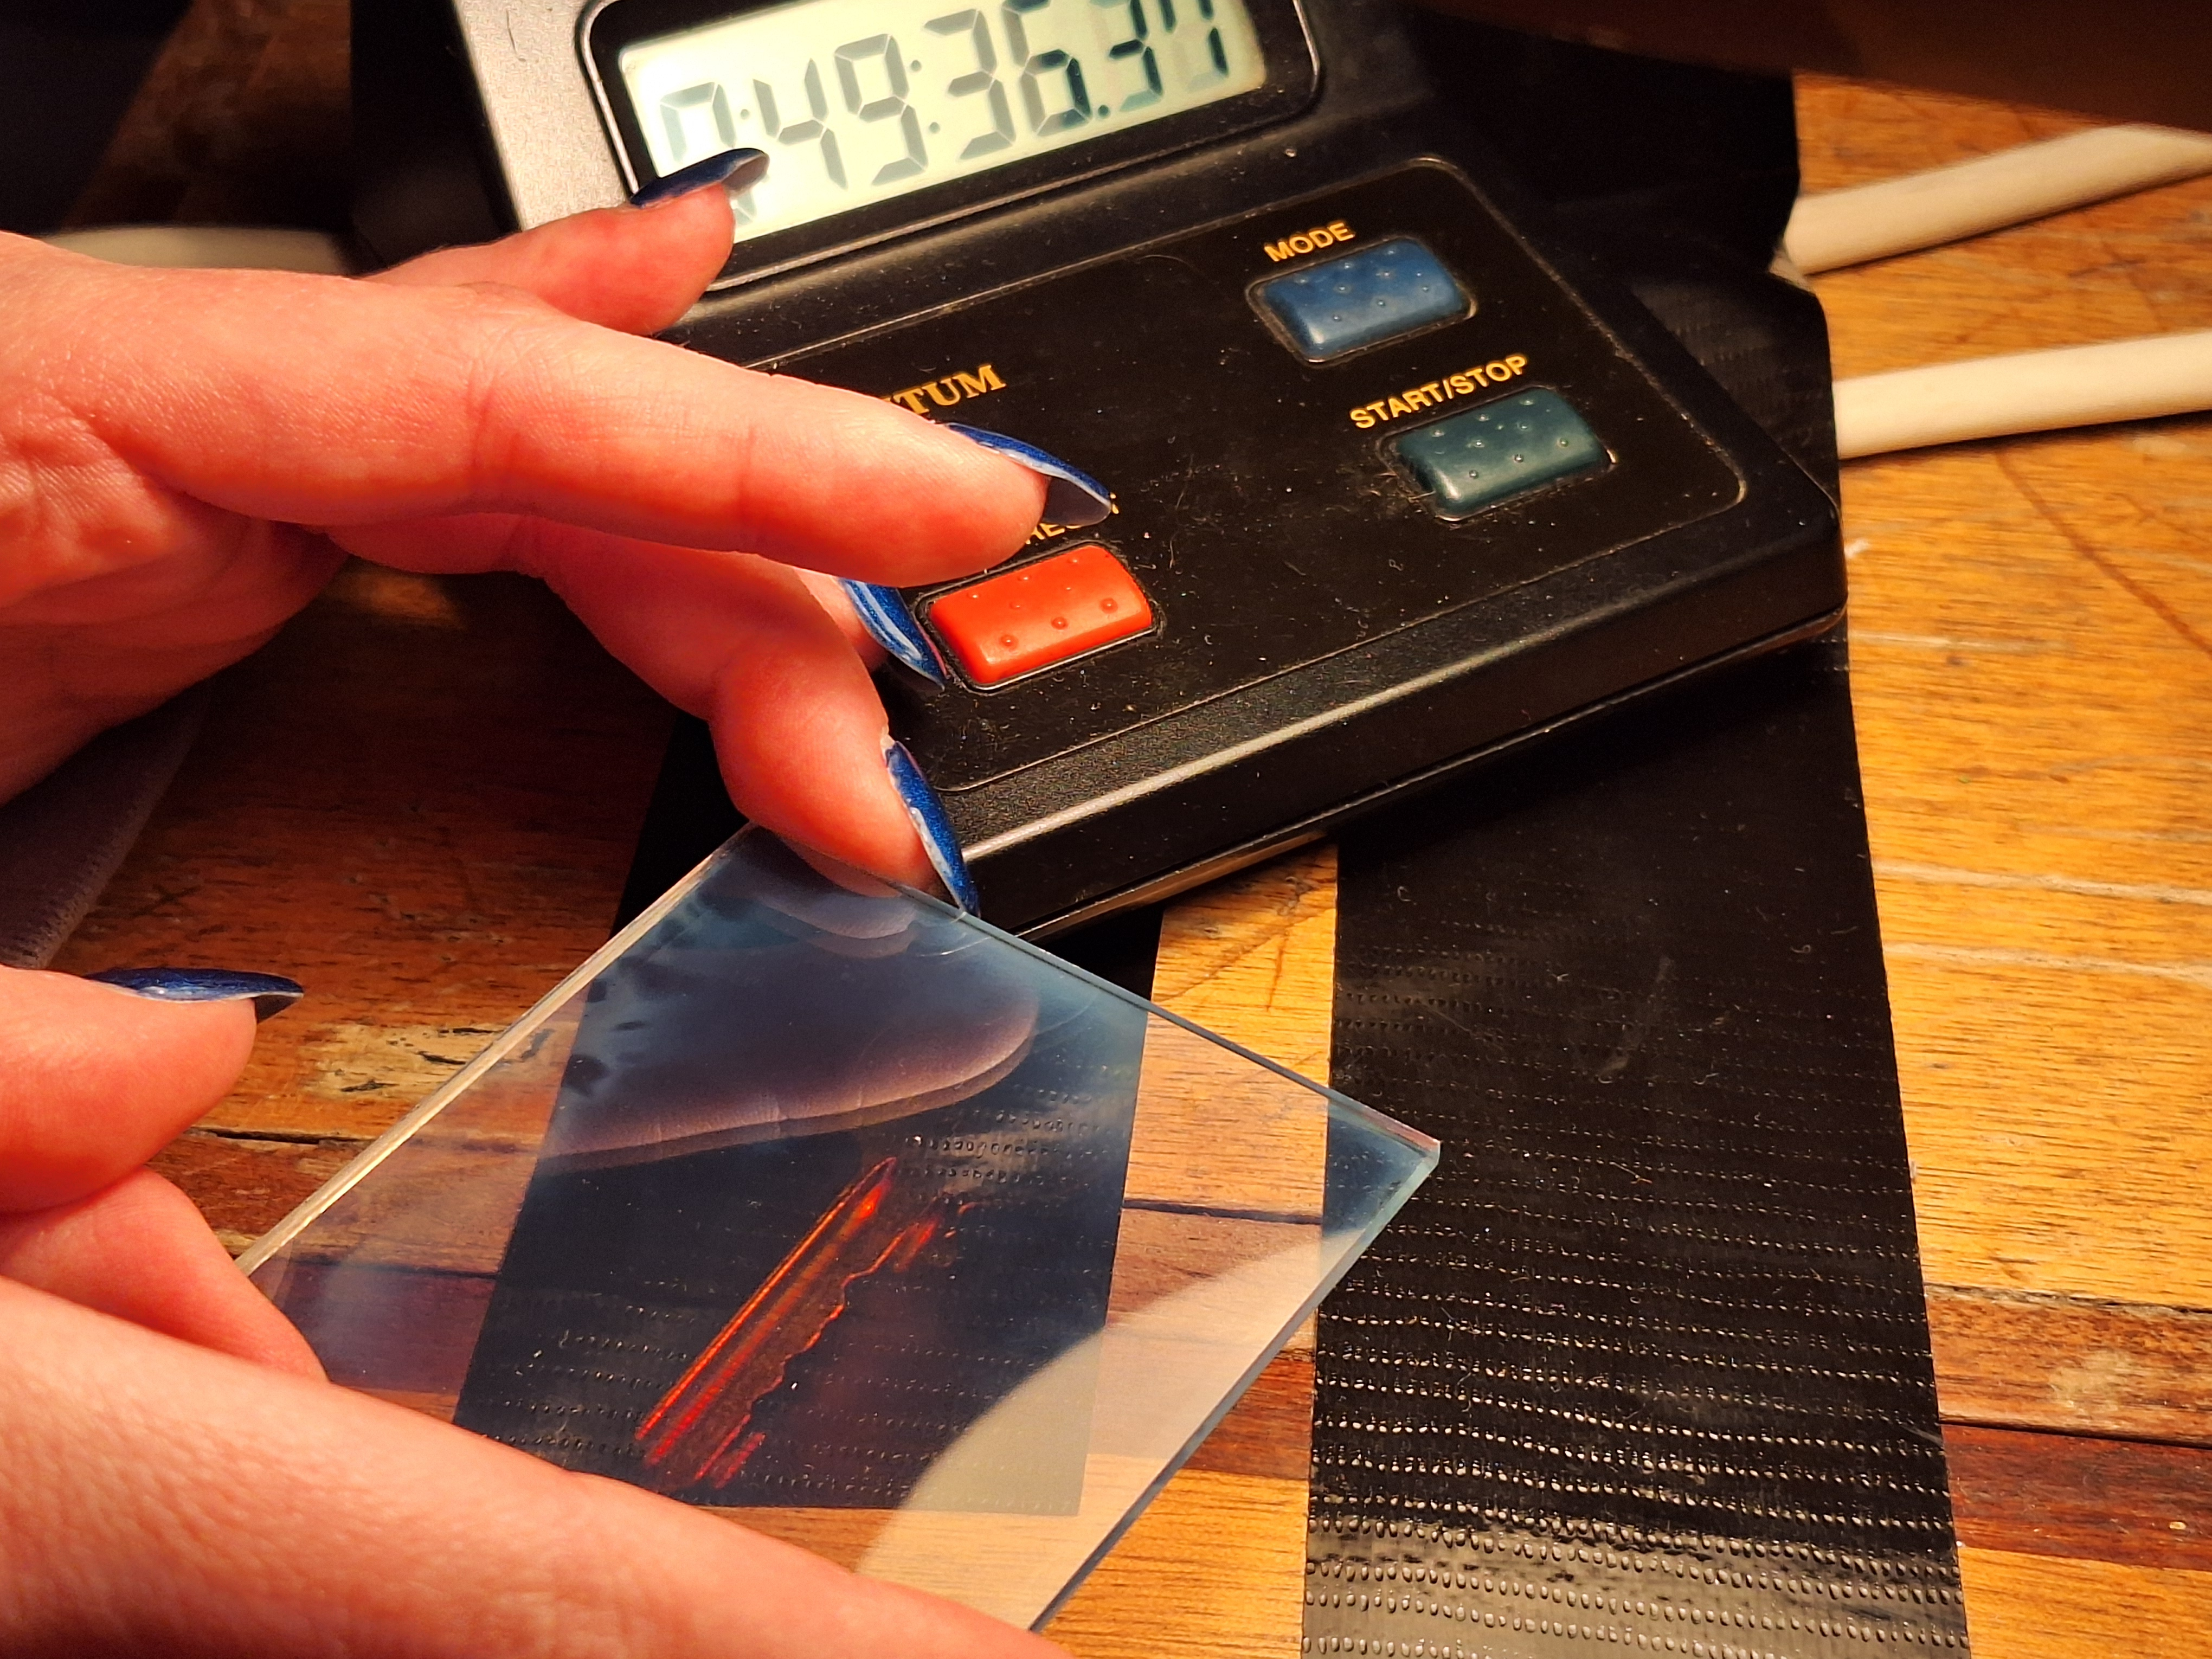
\includegraphics[width=\linewidth]{more red key.jpg}
    \end{minipage}
    \hspace{-.5em}
    \begin{minipage}{.452\textwidth}
        \includegraphics[width=\linewidth]{holo done 2 green.jpeg}
        \vfill
        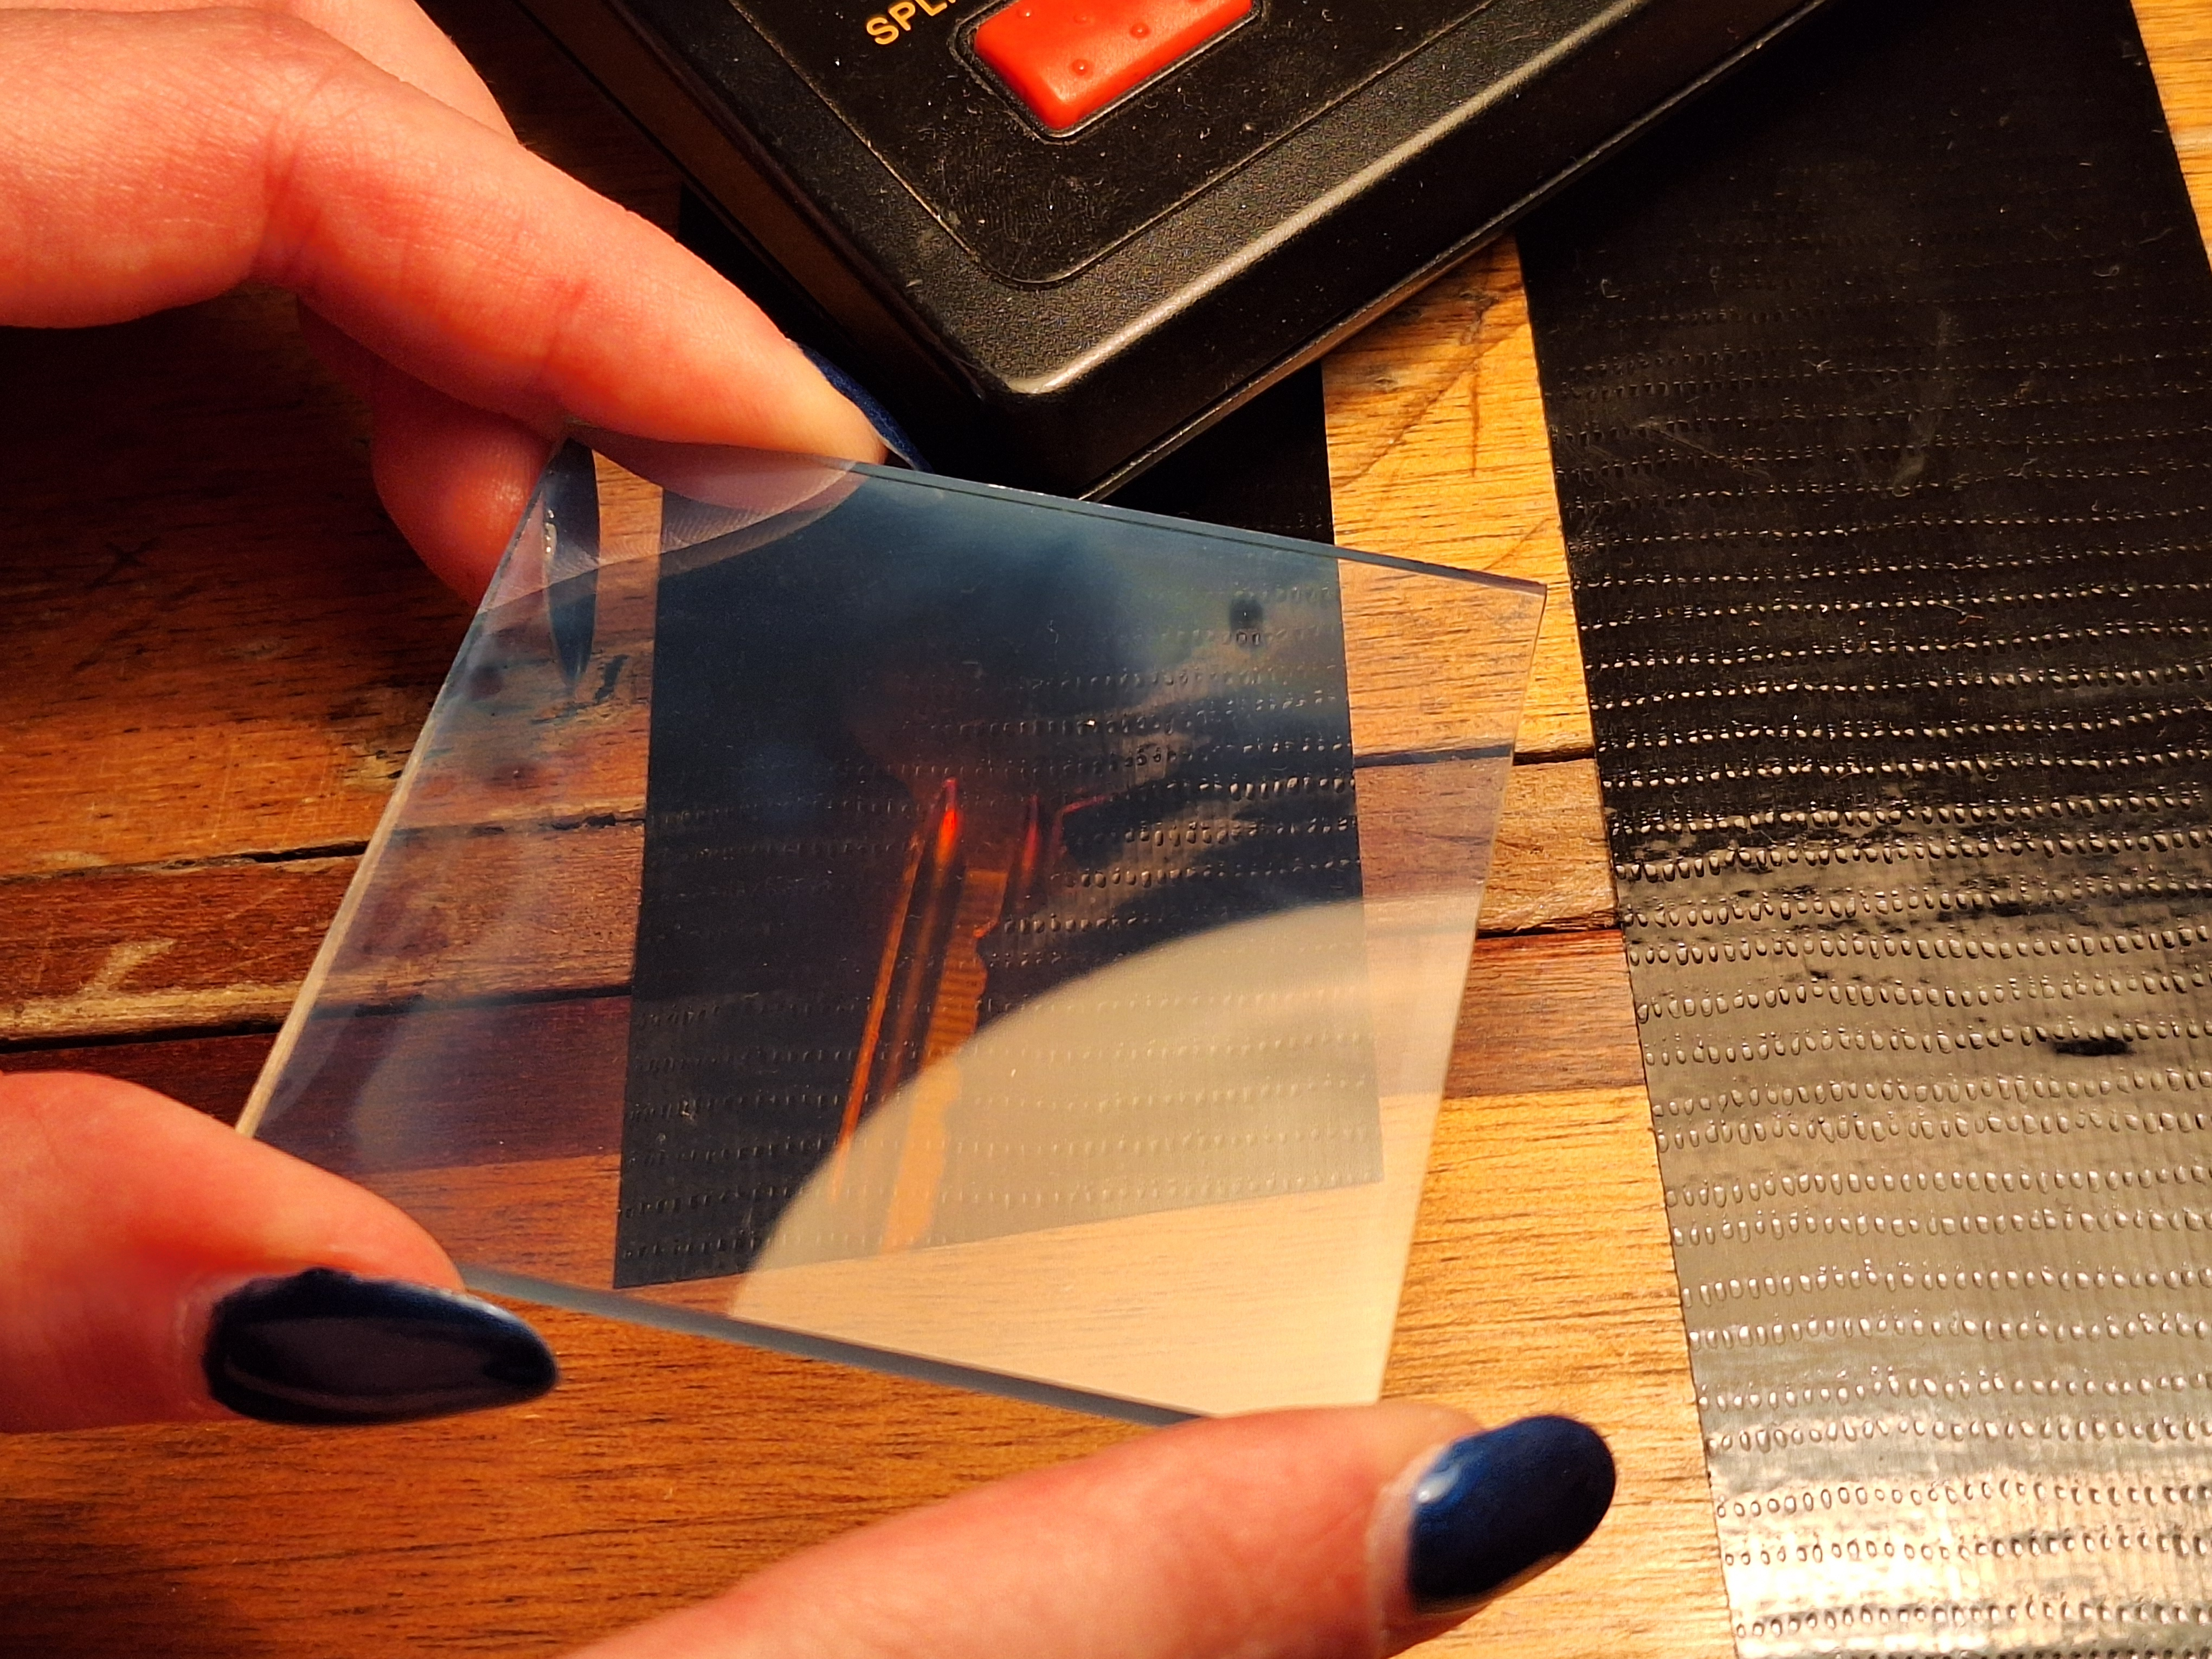
\includegraphics[width=\linewidth]{more key done but red.jpg}
    \end{minipage}
    \caption{\centering Reflection diagram of key final product.}
    \label{fig:13}
\end{figure}

As can be seen in Figure \ref{fig:13}, the full key was not captured. Particularly, the top of the circular head was not captured. The laser was clearly not fully positioned over the entire key, but as we wanted the room to be as dark as
possible we positioned everything in the dark and so were unable to verify if the key was completely illuminated. While the laser light was indeed a light source, the fact that it was red and so coherent it just resulted in headaches.
However, the fact that the part that wasn't recorded fades out rather than being a cut-off showcases the interacting behaviour of the light with the holographic plate. Additionally, while at most angles the key hologram is shown in the same colour
as the recording laser (red), there is a specific angle wherein it appears green instead (see Figure \ref{fig:13}, top right). This relates back to the fact that reflection holograms make use of Bragg diffraction in order to be seen in white light (see §\ref{sec:1.5.2}).

Despite the hologram appearing incredibly sharp and well-defined to the human eye, there were liekly some factors that, if avoided further, could have resulted in a higher quality hologram. It was decided to do all of the development of the hologram in the dark, just to make
sure there truly wasn't any accidental exposure until the hologram was fully developed in the chemicals, but this also meant that I was digging around the chemical containers in the dark looking for the edges of a near-invisible plate. This likely caused some scrathing on the emulsion surface.
As well, since I didn't want to stand in the dark room for the full 15 minuts of recording, I tried to leave as slowly and carefully as possible to minimise vibrations and outside light in as possible. Of course, I am still only human,
and it's likely there were still vibrations and light exposure. 

\section{Conclusion} \label{sec:4}

This experiment was successful in recording and reconstructing a hologram of a key with great clarity and sharpness, and thus also successfully desmonstrated the key concepts and principles explored in holography.
The final results of the hologram showed the strong correlation between the image quality of the hologram and influence factors discussed in the Theory section, such as alignment, laser coherence and monochromaticity, and minimal vibrations/outside exposure
during the recording process.

The final hologram clearly displayed the expected results of a well-defined 3D image reconstruction of the original object. A portion of the key was not captured due to errors in laser positioning during the recording process but all other
influencing factors appear to have been minimised as the resulting hologram was clear and sharp.

In future renditions of this experiment, greater care could be taken to further minimise vibrations and unwanted light exposure, as well as ensuring the laser is properly illuminating the full object so a well-rounded conclusion can be accomplished.
Greater care when processing the holographic emulsion plate in the chemicals can be considered to avoid possibly scratching the surface, and some light can be allowed into the darkroom during this process so the location of the holographic plate is not lost.

Despite shortcomings, this experiment was able to reaffirm the particular importance of using a laser light in holography due to its properties of monochromaticity, cohrerence, directionality, and intensity, as well as successfully displaying the effects of Bragg diffraction in
reflection holograms when viewing the hologram at parallax. These results also further emphasise the versatility of holography in all sectors of the world, particularly those discussed of medical imaging, data storage, and augmented/virtual reality devices.

\newpage

%%%%%%%%%%%%%%%%%%%%%%%%%%%%%%%%%%%

\bibliographystyle{IEEEtran}
\bibliography{References} \label{sec:ref}

\vspace{1.5cm}

\listoffigures


\end{document}